\documentclass[conference,letterpaper]{IEEEtran}
% Four technical pages and a reference-only fifth page. No margin/font shrinking.
\usepackage[T1]{fontenc}
\usepackage{newtxtext,newtxmath}
\usepackage{amsmath,booktabs,array,tabularx}
\usepackage{graphicx,tikz}
\usetikzlibrary{arrows.meta,positioning,calc}
\usepackage{cite}
\usepackage[hidelinks]{hyperref}
\usepackage{microtype}
\newcommand{\epl}{EP-L2}
\newcommand{\base}{B16}
\newcommand{\unif}{U-WB16}
\newcolumntype{L}[1]{>{\raggedright\arraybackslash}p{#1}}
% Real, fixed-height layout reservations. They intentionally contain no fake data.
\newcommand{\resultpanel}[4]{\fbox{\begin{minipage}[c][#2][c]{\dimexpr#1-2\fboxsep-2\fboxrule\relax}\centering
\small\textbf{#3}\par\medskip
\footnotesize MEASUREMENTS PENDING\par\medskip
\parbox{.91\linewidth}{\centering\footnotesize #4}
\end{minipage}}}
\hypersetup{pdftitle={EP-L2: Elastic Payload Storage for In-Place Writeback in GPU L2 Caches},pdfauthor={EP-L2 project; author information pending},pdfsubject={EN-v6 r21: verified writeback literature; frozen H0 results; separate r19 sensitivity}}
\hyphenation{write-back micro-ar-chi-tec-ture in-di-rec-tion}
\begin{document}
\title{EP-L2: Elastic Payload Storage for\\In-Place Writeback in GPU L2 Caches}
\author{\IEEEauthorblockN{Author information to be completed}\IEEEauthorblockA{English working draft EN-v6 (r21) --- not for submission}}
\maketitle
\begin{abstract}
A fixed-partition L2 may copy a dirty victim into a writeback buffer even though its data do not change. Elastic Payload L2 (EP-L2) retains the victim in place, separates tag visibility from payload ownership and writeback ordering, and allocates resident/writeback roles across a shared pool. We evaluate this WB-only mechanism against a fixed-partition reference with equal payload capacity and modeled bank service. Independent intake of five complete H0 native nonatomic workload pairs confirms removal of all resident-to-writeback copies. However, the geometric-mean execution-speed ratio is only 1.001600, with one slowdown; end-to-end performance is nearly unchanged. Three pressured workloads eliminate WB-data-full events while increasing downstream queue-admission denials. These observations motivate a controlled downstream-headroom study rather than establish its cause. The evidence covers symbolic sector versions and resource lifecycle, not numerical SASS outputs. Independent elasticity benefits, general workload speedup, and physical PPA advantages remain unestablished.
\end{abstract}
\begin{IEEEkeywords}
GPU, L2 cache, writeback, tag--data decoupling, resource sharing
\end{IEEEkeywords}

\section{Introduction}
A dirty eviction changes a line's consumer without changing its data. Our reference nevertheless copies it to a writeback buffer (WBUF), competing with demand accesses and fills. A full WBUF can block eviction despite idle storage elsewhere. Removing copy work helps only when other resources allow progress.

Prior designs already retain dirty data in the LLC and separately expose writeback candidates or dirty metadata~\cite{vwq,lastwrite,dbi}. Our question is narrower: can a resident tag be reused while its evicted dirty payload retains its original physical slot? \epl{} implements this transition with a legal incoming landing and distinct local-data and address-ordering release events, under fixed tag, payload, and bank-service budgets. Storage sharing alone is not the proposed contribution.

Five matched pairs remove copies but yield only a 0.160\% geometric-mean speed-ratio gain. Strong static controls must isolate elasticity from copy removal; concurrent bypass and TVD/RO are outside this WB-only comparison.

\section{EP-L2 Design}
\subsection{One-Slice Organization and Comparison Boundary}
The primary reference, \base{} (\texttt{B16\_BANKED}), partitions 1168 line-sized slots into 1024 resident, 128 bypass-return, and 16 WBUF slots. \unif{} (\texttt{U\_WB16}) permits resident and WB allocations across this physical pool. Each slot is 128 B with four 32-B sectors. Both modes provision four banks of 292 slots, at most one modeled line-sized operation per bank per physical GPU cycle, and a common 128-B copy latch outside the pool. Both also retain 128 writeback address-directory (WAD) entries and the same request-metadata limits. Sixteen is the static \emph{data} quota, not the U-WB control limit.

\begin{figure*}[t]
\centering
\begin{minipage}[t]{.49\textwidth}
\centering\small\textbf{(a) Logical organization of one L2 slice}\par\smallskip
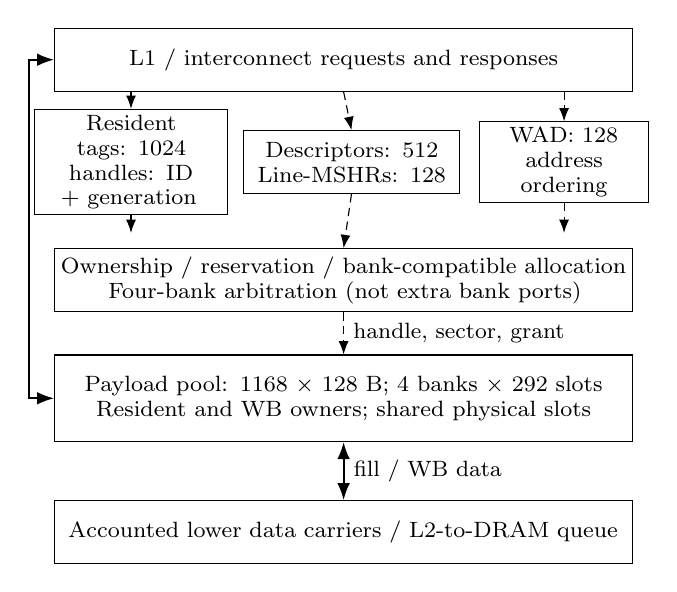
\begin{tikzpicture}[x=1mm,y=1mm,>=Latex,font=\fontsize{8}{9}\selectfont,
box/.style={draw,align=center,inner sep=2pt,minimum height=8mm},
ctl/.style={->,densely dashed,line width=.4pt},data/.style={<->,line width=.7pt}]
\node[box,text width=72mm] (in) at (40,53) {L1 / interconnect requests and responses};
\node[box,text width=23mm] (tag) at (13,40) {Resident tags: 1024\\handles: ID + generation};
\node[box,text width=26mm] (req) at (41,40) {Descriptors: 512\\Line-MSHRs: 128};
\node[box,text width=20mm] (wad) at (68,40) {WAD: 128\\address ordering};
\node[box,text width=72mm] (ctrl) at (40,25) {Ownership / reservation / bank-compatible allocation\\Four-bank arbitration (not extra bank ports)};
\node[box,text width=72mm,minimum height=11mm] (pool) at (40,10) {Payload pool: 1168 $\times$ 128 B; 4 banks $\times$ 292 slots\\Resident and WB owners; shared physical slots};
\node[box,text width=72mm] (low) at (40,-7) {Accounted lower data carriers / L2-to-DRAM queue};
\draw[ctl] (in.south)--(req.north);
\draw[ctl] (13,49)--(tag.north);\draw[ctl] (68,49)--(wad.north);
\draw[ctl] (tag.south)--(13,31);\draw[ctl] (req.south)--(ctrl.north);\draw[ctl] (wad.south)--(68,31);
\draw[ctl] (ctrl.south)--node[right]{handle, sector, grant} (pool.north);
\draw[data] (pool.south)--node[right]{fill / WB data} (low.north);
\draw[data] (in.west)--(0,53)--(0,10)--(pool.west);

\end{tikzpicture}
\end{minipage}\hfill
\begin{minipage}[t]{.49\textwidth}
\centering\small\textbf{(b) Copy removal and separate release events}\par\smallskip
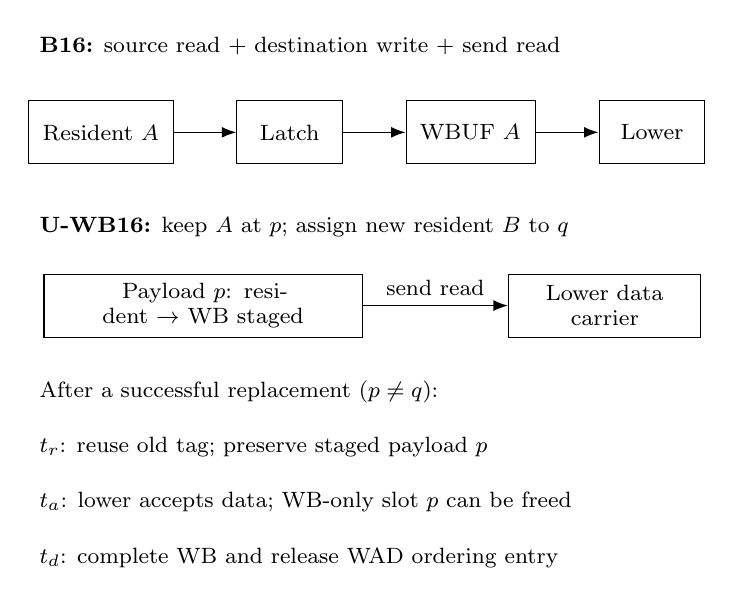
\begin{tikzpicture}[x=1mm,y=1mm,>=Latex,font=\fontsize{8}{9}\selectfont,
box/.style={draw,align=center,inner sep=2pt,minimum height=8mm},arr/.style={->,line width=.5pt}]
\node[anchor=west] at (0,55) {\textbf{B16:} source read $+$ destination write $+$ send read};
\node[box,text width=17mm] (a) at (9,44) {Resident $A$};
\node[box,text width=12mm] (l) at (33,44) {Latch};
\node[box,text width=15mm] (w) at (56,44) {WBUF $A$};
\node[box,text width=12mm] (d) at (79,44) {Lower};
\draw[arr] (a)--(l);\draw[arr] (l)--(w);\draw[arr] (w)--(d);
\node[anchor=west] at (0,32) {\textbf{U-WB16:} keep $A$ at $p$; assign new resident $B$ to $q$};
\node[box,text width=39mm] (p) at (22,22) {Payload $p$: resident $\to$ WB staged};
\node[box,text width=23mm] (lo) at (73,22) {Lower data carrier};
\draw[arr] (p)--node[above]{send read} (lo);
\node[anchor=west] at (0,11) {After a successful replacement ($p\ne q$):};
\node[anchor=west] at (0,4) {$t_r$: reuse old tag; preserve staged payload $p$};
\node[anchor=west] at (0,-3) {$t_a$: lower accepts data; WB-only slot $p$ can be freed};
\node[anchor=west] at (0,-10) {$t_d$: complete WB and release WAD ordering entry};
\end{tikzpicture}
\end{minipage}
\caption{Declared WB-only design, not a physical floorplan or a measured cycle schedule. Dashed links denote control dependencies; solid links denote data movement. B16 uses fixed 1024/128/16 role quotas over the same banks; U-WB16 allows resident/WB allocation across those slots. Concurrent dynamic bypass service is not established. Both retain a 128-B copy latch outside the pool. Optional TVD/RO consumers are not drawn as extra data arrays.}
\label{fig:organization}
\end{figure*}


Figure~\ref{fig:organization} shows the declared service model. WB-only pooling can borrow reference bypass-return slots, but concurrent dynamic bypass use is unvalidated. Idle bypass capacity therefore makes a WB-heavy static control important.

A resident tag names a payload through a slot identifier and generation. Each slot has one authoritative owner; ready/pending sector masks and pins track its consumers. The initial design preserves the resident bank class:
\begin{equation}
 \operatorname{bank}(p)=p\bmod4=\operatorname{tag\_index}\bmod4.
\label{eq:bank}
\end{equation}
A globally free slot is therefore not necessarily a legal landing for a given tag. The 1024 tags bound resident visibility; a temporarily reserved incoming landing is not an additional visible resident line.

\subsection{Replacement as a Transaction}
Before a dirty replacement commits, the controller obtains the address-ordering entry, required issue resources, and a legal landing. In B16, it reads the victim into the latch and writes WBUF before reusing the resident slot. In U-WB16, dirty line $A$ remains in payload $p$ as \texttt{WB\_STAGED}; new resident $B$ receives $q\ne p$. The send read and lower data carrier remain necessary in both modes.

Precheck refusals acquire no visible ownership; bank retries may retain reservations across cycles. The reserved victim, requester, and eventual native tag commit must agree. If an intervening fill changes a subsequent victim selection, the controller must preserve the original transaction or fully roll it back before preparing another. Rollback releases reservations, not bank work already performed.

The repaired release passes producer and independent directed qualification, including the tested cross-cycle boundary. Application qualification remains bounded by the native nonatomic scope below.

\subsection{Separate Release Events}
At committed replacement time $t_r$, the old tag can be reused. Payload $p$ remains protected until actual downstream data acceptance $t_a$. The WAD retains same-address ordering until writeback completion $t_d$. A software queue pointer alone does not constitute a data handoff: a separately accounted lower carrier must own the dirty data before local staging is released. A late event for $A$ uses its own handle/transaction identity, not the tag now naming $B$.

For tracked reads, requester descriptors and payload pins remain live until response-queue acceptance or internal consumption. Line-MSHR retirement and pending-sector completion are checked separately. Neither event releases a WB address-ordering obligation. A read of one ready sector does not imply that an entire line is ready. Atomic and ordinary requests sharing a line additionally require sector-appropriate dirty and version handling.

Local drain progress requires both eventual lower service and a bank retry that remains identifiable until completion or explicit cancellation. An oldest-selected grant alone cannot guarantee progress if its requester changes identity or stops retrying. Whole-GPU deadlock freedom is not established by these local requirements.

\begin{figure*}[t]
\centering
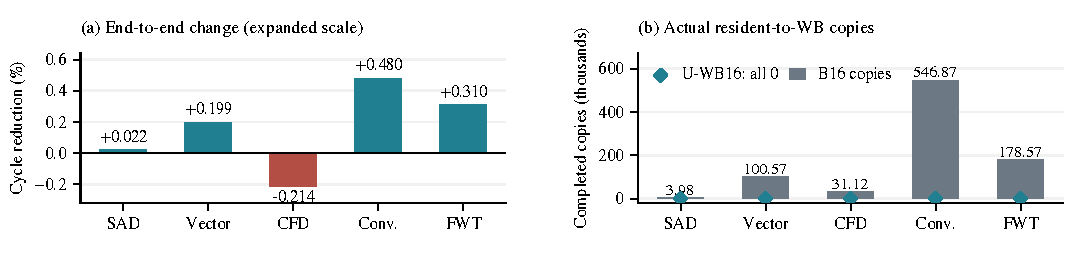
\includegraphics[width=\textwidth]{figures/fig2_results.pdf}
\caption{Five independently received H0 native pairs, unchanged by diagnostic conditions. (a) Cycle reduction $100(C_B-C_U)/C_B$, on an expanded scale with zero denoting B16; CFD regression is retained. The speed-ratio geomean is 1.001600, not the mean of these percentages. (b) Actual completed 128-B copies; U-WB16 is zero in every pair. Vector, Conv., and FWT denote vectorAdd\_4M, convolutionSeparable, and FWT\_7\_21. No error bars or significance claim.}
\label{fig:mainresults}
\end{figure*}

\subsection{Implementation Cost and Separate Extensions}
Primary payload storage is 146 KiB/slice, or 9.125 MiB over 64 slices; common latches add 8 KiB/chip. A slot index requires $P=11$ bits. Explicit tag handles occupy $1024(P+G)$ bits for generation width $G$; up to 128 WB handles require $128(P+G)$ bits plus state and transaction binding. These are gross representations, not measured incremental area: the reference already includes some common fields.

Incremental cost includes handle selection, owner/generation checks, bank-compatible allocation, arbitration, and rollback. Queue depths, generation/pin bounds, pipeline stages, SRAM ports, and the carrier after $t_a$ need concrete mappings. Symbolic versions are verification state, not payload RAM. Equal capacity/throughput does not prove equal hit latency, area, clock, or energy. No RTL synthesis, STA, or power measurement is available.

TVD retains displaced payloads within a shared 128-entry WAD/TVD budget. RO controls pending-tag detachment and Line-MSHR bypass under a whole-commandlist read-only oracle. Both are OFF here. TVD lacks official integrated qualification; RO has isolated source-bound C++ checks, but its 19 production obligations and independent scientific qualification remain pending. Neither has accepted application results or an extra data/descriptor pool.

\section{Evaluation Methodology}
\subsection{Matched Inputs and Declared Machine}
We use the Accel-Sim SASS flow and GPGPU-Sim performance-model lineage~\cite{accelsim,gpgpusim}. Their published validation does not validate this modified L2. B16 and U-WB16 must execute with the same independently qualified binary, complete trace input, non-mode settings, timing scope, and termination rules. Table~\ref{tab:configuration} records the current ordered research configuration, including the modified L2; it is not a reconstruction of undocumented commercial-cache internals.

\begin{table}[t]
\caption{Declared matched configuration. L2 capacities are per slice.}
\label{tab:configuration}\centering\footnotesize
\begin{tabularx}{\columnwidth}{@{}L{.42\columnwidth}X@{}}
\toprule
Resource & Setting \\
\midrule
Compute / clock domains & 80 SMs; core/ICNT/L2: 1132 MHz; DRAM: 850 MHz \\
L1 (fixed) & 64 KiB/SM; 4 banks; 20-cycle setting \\
L2 tags / data & 1024 tags; 1168 slots, 146 KiB \\
Line / sectors / banks & 128 B / $4\times32$ B / $4\times292$ slots \\
Service / common latch & 1 op/bank/physical cycle / 128 B \\
Descriptors / Line-MSHRs & 512 / 128; 32 requesters/address \\
WAD / lower queue & 128 / 128 entries \\
Chip / memory channels & 64 slices / 32 channels \\
L2 ROP delay & 160-cycle model setting \\
DRAM scheduler / return & 128 / 192 entries per channel \\
WBUF8 (not evaluated) & 1160 slots, 145 KiB; $4\times290$ slots \\
\bottomrule
\end{tabularx}
\end{table}

The fixed development set is convolutionSeparable, FWT\_7\_21, cfd\_097k, vectorAdd\_4M, and SAD. Accepted manifests bind each complete commandlist, input size, and trace body; workload names alone are insufficient. SAD is the predeclared negative control. All five pairs, including slowdowns, enter the geometric mean. This development set does not establish holdout or general GPU coverage.

\subsection{Correctness Before Performance}
The repaired producer and its independent replay each pass 31 directed invocations, and Lane5 accepts the complete eleven-gate protocol. Per-spec complete-content proofs restrict application qualification to native nonatomic inputs. New results remain bound to the exact source, binary, configurations, and input content.

Qualification covers host-prefill identity, physical-cycle grants, generation reuse, partial/out-of-order sectors, response backpressure, and separate WB acceptance/completion. Native tag time may include a host-copy offset; bank service must use the physical clock. Nonatomic results do not qualify mixed atomic workloads.

SASS traces do not supply complete numerical payloads. The supported checks concern ownership, symbolic sector versions, requester/transaction identity, and resource drain; they are not full numerical application verification. The independent paper intake rehashes full native trace bodies, executable, ordered configurations, and raw logs, reparses all 64 slice terminals with the producing parser, and checks the current withdrawal authority. Legacy zero-mask records remain in the original inputs under a source-bound native-byte semantic proof; no rows are removed. Historical PASS cannot override a later scientific withdrawal.

\section{Results and Causal Analysis}
\subsection{Performance and Internal Movement}
All five predeclared H0 pairs pass independent paper intake against the current Lane5 V2 authority. Each pair has equal instruction counts and matched full input/termination scope. Figure~\ref{fig:mainresults}(a) reports the complete set: SAD is almost tied; Vector, Convolution, and FWT reduce cycles by 0.199\%, 0.480\%, and 0.310\%, while CFD increases cycles by 0.214\%. The geometric mean of $C_B/C_U$ is 1.001600, or a 0.160\% speed-ratio gain. These deterministic paired observations establish neither statistical significance nor general GPU speedup. Exact paired cycles and source/configuration/input/raw identities accompany the artifact tables.

Figure~\ref{fig:mainresults}(b) shows removal of every measured resident-to-WB copy. A committed non-rolled-back B16 writeback uses two copy operations and one send read; U-WB16 retains the send read. This local operation saving is not a speedup model. Actual WB counts also change: CFD completes 31,123/31,063 WBs and FWT 178,569/178,585 for B16/U-WB16. Consequently, the run-level logical-operation difference need not equal twice either mode's WB count. Artifact tables preserve actual WB/send-read and DRAM-byte totals.

\begin{figure*}[t]
\centering
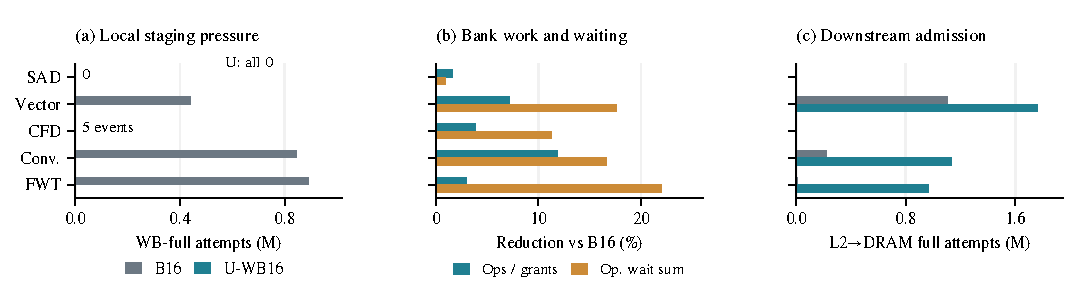
\includegraphics[width=\textwidth]{figures/fig3_pressure.pdf}
\caption{H0 application-cumulative pressure and service observations. (a) WB-data-full refusal attempts; CFD's small B16 count is labeled explicitly. (b) Separate relative reductions in logical work/successful modeled bank grants and in summed per-operation conflict waits. Logical operations and grants coincide at drain in these runs, but are independently checked counters. (c) Frontend attempts denied when the L2-to-DRAM queue is full. M denotes $10^6$. Attempt counts and operation-wait sums are not elapsed GPU cycles or unique transactions; reductions and increases do not establish causality.}
\label{fig:causal}
\end{figure*}

\subsection{Local Pressure and Downstream Service}
Vector, Convolution, and FWT record 440,161, 845,097, and 890,294 B16 WB-data-full events; U-WB16 records zero. Figure~\ref{fig:causal}(b) shows less modeled bank work and lower aggregate conflict waits. Successful grants are actual model-service observations, not estimates obtained by multiplying copies. At drained termination, their equality to logical operations implies neither elapsed-time nor RTL timing/energy savings.

For the same three workloads, L2-to-DRAM full-block attempts rise from 1.104M to 1.764M, 0.218M to 1.132M, and 0.013M to 0.968M. This is consistent with pressure moving downstream after local staging relief. It does not independently identify the limiting queue or DRAM service. Denials may repeat for one frontend head and overlap other blockers. From final cumulative observations of all 32 channels, the modeled issued-byte/atom-cycle fractions are 64.5/64.8\% for Convolution and 14.1/14.1\% for FWT. Even frequent queue denials therefore do not prove global DRAM-bandwidth saturation. Kernel-boundary cumulative snapshots are not summed.

CFD is a useful counterexample: despite removing copies and lowering bank waits from 102,546 to 91,029, U-WB16 takes 169 more cycles. WAD-hazard events increase from 9,841 to 13,400, WB counts differ, and successful DRAM writes change from 3,983,744 to 3,976,064~B. These correlated changes motivate ordering/service diagnosis; they do not identify a unique cause. SAD has no observed WB-data-full pressure and differs by only 24 cycles. Neither case is discarded.

\begin{figure}[t]
\centering\footnotesize
\begin{tabular}{@{}lrr@{}}
\toprule
Condition & Target DRAM MHz & Accepted B/U pairs \\
\midrule
H0 (reused) & 850 & $2/2$ \\
Q4 & 850 & $0/2$ \\
D4 & 3400 & $0/2$ \\
\bottomrule
\end{tabular}
\caption{Authorized r19 targets for Convolution/FWT. Q4/D4 lack published qualified native pairs at this snapshot. Counts are accepted pairs, not performance. H0 five-workload results remain unchanged.}
\label{fig:controls}
\end{figure}

\subsection{Downstream Service Sensitivity and Interaction}
R19 authorizes Convolution/FWT under H0, Q4, and D4, with D4 pairs first. For each condition $h$, define
\begin{equation}
 S(h)=C_B(h)/C_U(h),\qquad J(h)=S(h)/S(\mathrm{H0}).
\end{equation}
Retain all four cycles and absolute changes. $C_B(\mathrm{H0})/C_U(h)$ confounds mechanism and downstream changes. Diagnostic results never enter the H0 mean.

Q4 enlarges downstream queues, scheduler/return storage, and derived credit $319\to1279$. Request buffers also affect scheduling visibility and implementation complexity~\cite{sms}. D4 retains Q4 buffering and raises DRAM $850\to3400$\,MHz, with core/ICNT/L2 fixed at 1132\,MHz. Integer DRAM timings shorten physically; the fixed 100-GPU-cycle interface delay remains. These are grouped buffering/credit and DRAM-domain interventions, not pure bandwidth or free hardware.

Figure~\ref{fig:controls} tracks accepted-pair coverage. New pairs require exact regime/configuration identity and current V2/native closure. Interpret $J$ with copy work, residence, bank service, valid opportunity ratios, and queue maxima. Faster service can shorten B16 WB residence, so $S$ need not rise monotonically. SMS does not establish EP-L2's bottleneck. Adaptive points need an evidence checkpoint; simple-memory diagnostics require separate qualification.

An equal 1168-slot strong static control remains unqualified; B16/U combines copy removal and pooling. WBUF8 has 1160 slots. TVD/RO/Ideal and physical PPA remain separate gaps.

\section{Related Work and Scope}
The Virtual Write Queue exposes LLC dirty-line candidates to DRAM scheduling while retaining a physical write queue~\cite{vwq}. Decoupled last-write prediction keeps candidate addresses in a last-write buffer and data in the LLC; evicted dirty blocks use a separate write buffer~\cite{lastwrite}. The Dirty-Block Index (DBI) separates dirty bits from tags and groups them by DRAM row~\cite{dbi}. Neither cache retention nor independent dirty metadata originates here. Our focus is tag reuse with the victim's original slot still owned, a distinct incoming landing, and separate payload/order retirement. DBI dirty status is not the WAD's in-flight same-address ordering state.

V-Way decouples tag/data placement~\cite{vway}; Tag-Split Cache separates request and storage granularity~\cite{tsc}. Unified GPU memory reallocates SM register/cache/scratchpad storage~\cite{unified}. In-cache MSHRs~\cite{farkas}, MiCache's shared FPGA data/MSHR storage~\cite{micache}, and DL-MSHR's linked slots, including write-miss data~\cite{dlmshr}, motivate distinguishing what is shared. Our comparison fixes resident-tag and miss-tracking budgets; it evaluates dirty-payload ownership rather than extra lookup or request-tracking capacity.

\section{Conclusion}
\epl{} separates resident-tag visibility, dirty-payload ownership, and writeback ordering to eliminate resident-to-WB relocation under a fixed payload and bank-service budget. Five independently received native nonatomic pairs remove all measured copies but deliver only a 1.001600 geometric-mean speed ratio, including a CFD slowdown. Local staging relief coincides with more downstream admission denials in three workloads; a controlled service study is required to resolve causality. Independent elasticity benefits and physical area, timing, and power advantages remain unproven.

% Keep the optional fifth page reference-only. No technical appendix on that page.
\clearpage
\bibliographystyle{IEEEtran}
\bibliography{references_verified}
\end{document}
